% Figura 2: Diagrama de Orthogonalización
% Muestra el proceso de eliminación de la dirección de rechazo
%
% Compilar con: pdflatex fig2_orthogonalization.tex
%
\documentclass[12pt]{article}
\usepackage[paperwidth=20cm,paperheight=15cm,margin=0.5cm]{geometry}
\usepackage{tikz}
\pagestyle{empty}
\usepackage{amsmath}
\usepackage{amssymb}
\usetikzlibrary{arrows.meta, calc, decorations.pathmorphing, positioning, shapes.geometric, 3d}

% Colores
\definecolor{refusalred}{RGB}{214,39,40}
\definecolor{harmlessgreen}{RGB}{44,160,44}
\definecolor{directionblue}{RGB}{31,119,180}
\definecolor{modifiedpurple}{RGB}{148,103,189}
\definecolor{weightgray}{RGB}{127,127,127}

\begin{document}
\centering
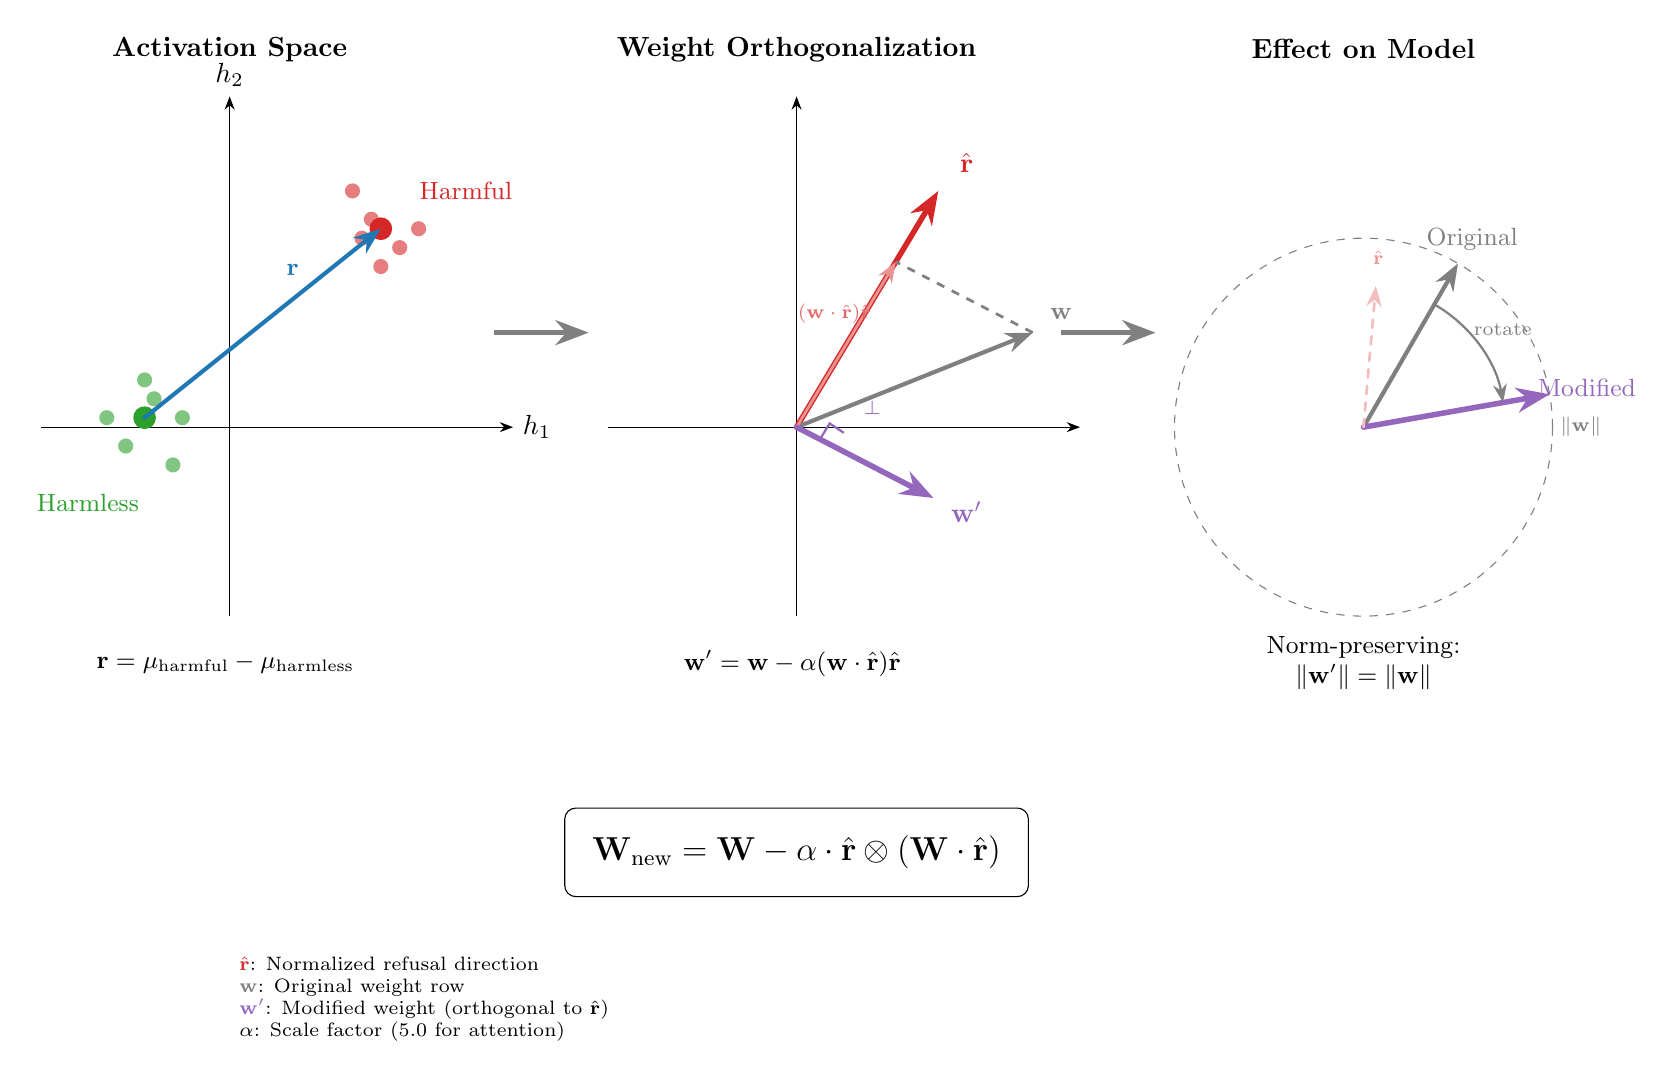
\begin{tikzpicture}[
    scale=1.2,
    >=Stealth,
    vector/.style={->, thick, line cap=round},
    projection/.style={dashed, gray},
    label/.style={font=\small},
]

% === PANEL IZQUIERDO: Espacio de Activaciones ===
\begin{scope}[shift={(-6,0)}]
    % Título
    \node[font=\bfseries] at (0,4) {Activation Space};

    % Ejes
    \draw[->] (-2,0) -- (3,0) node[right] {$h_1$};
    \draw[->] (0,-2) -- (0,3.5) node[above] {$h_2$};

    % Cluster harmless (verde)
    \foreach \x/\y in {-0.8/0.3, -1.1/-0.2, -0.6/-0.4, -1.3/0.1, -0.9/0.5, -0.5/0.1} {
        \fill[harmlessgreen, opacity=0.6] (\x,\y) circle (0.08);
    }
    \node[harmlessgreen, font=\small] at (-1.5,-0.8) {Harmless};

    % Cluster harmful (rojo)
    \foreach \x/\y in {1.5/2.2, 1.8/1.9, 1.3/2.5, 2.0/2.1, 1.6/1.7, 1.4/2.0} {
        \fill[refusalred, opacity=0.6] (\x,\y) circle (0.08);
    }
    \node[refusalred, font=\small] at (2.5,2.5) {Harmful};

    % Centroides
    \fill[harmlessgreen] (-0.9,0.1) circle (0.12);
    \fill[refusalred] (1.6,2.1) circle (0.12);

    % Refusal direction
    \draw[vector, directionblue, line width=1.5pt] (-0.9,0.1) -- (1.6,2.1);
    \node[directionblue, font=\small\bfseries, anchor=south west] at (0.5,1.5) {$\mathbf{r}$};

    % Fórmula
    \node[font=\small, align=center] at (0,-2.5) {
        $\mathbf{r} = \mu_{\text{harmful}} - \mu_{\text{harmless}}$
    };
\end{scope}

% === PANEL CENTRAL: Orthogonalización ===
\begin{scope}
    % Título
    \node[font=\bfseries] at (0,4) {Weight Orthogonalization};

    % Espacio de pesos original
    \draw[->] (-2,0) -- (3,0) node[right] {};
    \draw[->] (0,-2) -- (0,3.5) node[above] {};

    % Vector v (refusal direction normalizado)
    \draw[vector, refusalred, line width=2pt] (0,0) -- (1.5,2.5);
    \node[refusalred, font=\bfseries] at (1.8,2.8) {$\hat{\mathbf{r}}$};

    % Vector de peso original W
    \draw[vector, weightgray, line width=1.5pt] (0,0) -- (2.5,1);
    \node[weightgray, font=\small] at (2.8,1.2) {$\mathbf{w}$};

    % Proyección de W en r
    \coordinate (proj) at (1.05,1.75);
    \draw[projection, line width=1pt] (2.5,1) -- (proj);
    \draw[vector, refusalred!50, line width=1pt] (0,0) -- (proj);
    \node[refusalred!70, font=\scriptsize] at (0.4,1.2) {$(\mathbf{w} \cdot \hat{\mathbf{r}})\hat{\mathbf{r}}$};

    % Vector de peso modificado
    \draw[vector, modifiedpurple, line width=2pt] (0,0) -- (1.45,-0.75);
    \node[modifiedpurple, font=\bfseries] at (1.8,-0.9) {$\mathbf{w}'$};

    % Indicador de ortogonalidad
    \draw[modifiedpurple, thick] (0.25,-0.125) -- (0.35,0.04) -- (0.5,-0.06);
    \node[modifiedpurple, font=\scriptsize] at (0.8,0.2) {$\perp$};

    % Fórmula
    \node[font=\small, align=center] at (0,-2.5) {
        $\mathbf{w}' = \mathbf{w} - \alpha (\mathbf{w} \cdot \hat{\mathbf{r}})\hat{\mathbf{r}}$
    };
\end{scope}

% === PANEL DERECHO: Efecto en el Modelo ===
\begin{scope}[shift={(6,0)}]
    % Título
    \node[font=\bfseries] at (0,4) {Effect on Model};

    % Círculo de norma preservada
    \draw[gray, dashed] (0,0) circle (2);
    \node[gray, font=\scriptsize] at (2.3,0) {$\|\mathbf{w}\|$};

    % Vector original
    \draw[vector, weightgray, line width=1.5pt] (0,0) -- (60:2);
    \node[weightgray, font=\small] at (60:2.3) {Original};

    % Vector modificado (misma norma)
    \draw[vector, modifiedpurple, line width=2pt] (0,0) -- (10:2);
    \node[modifiedpurple, font=\small] at (10:2.4) {Modified};

    % Refusal direction (a eliminar)
    \draw[vector, refusalred!30, line width=1pt, dashed] (0,0) -- (85:1.5);
    \node[refusalred!50, font=\scriptsize] at (85:1.8) {$\hat{\mathbf{r}}$};

    % Arco mostrando rotación
    \draw[->, gray, thick] (60:1.5) arc (60:10:1.5);
    \node[gray, font=\scriptsize] at (35:1.8) {rotate};

    % Norm-preserving annotation
    \node[font=\small, align=center] at (0,-2.5) {
        Norm-preserving:\\
        $\|\mathbf{w}'\| = \|\mathbf{w}\|$
    };
\end{scope}

% === FLECHAS DE PROCESO ===
\draw[->, line width=2pt, gray] (-3.2,1) -- (-2.2,1);
\draw[->, line width=2pt, gray] (2.8,1) -- (3.8,1);

% === ECUACIÓN PRINCIPAL ===
\node[draw, rounded corners, fill=white, font=\large, inner sep=10pt] at (0,-4.5) {
    $\mathbf{W}_{\text{new}} = \mathbf{W} - \alpha \cdot \hat{\mathbf{r}} \otimes (\mathbf{W} \cdot \hat{\mathbf{r}})$
};

% === LEYENDA ===
\node[font=\scriptsize, align=left, anchor=north west] at (-6,-5.5) {
    \textcolor{refusalred}{$\hat{\mathbf{r}}$}: Normalized refusal direction\\
    \textcolor{weightgray}{$\mathbf{w}$}: Original weight row\\
    \textcolor{modifiedpurple}{$\mathbf{w}'$}: Modified weight (orthogonal to $\hat{\mathbf{r}}$)\\
    $\alpha$: Scale factor (5.0 for attention)
};

\end{tikzpicture}
\end{document}
